\chapter{Erweiterte Funktionen}
\section{Das Tag-Konzept von PUMA}
PUMA wird über \tags verwaltet. Mit Hilfe der \tags können Einträge verwaltet und sortiert werden.
\subsection{Tags}
\label{subsec:tags}
\tags\index{Tags} (dt. Schlagwörter) ermöglichen ein übersichtliches Organisieren und Strukturieren der Lesezeichen. Einem Literatureintrag können beliebig viele \tags zugeordnet werden. Durch den Gebrauch von \tags wird die Suche zu einem bestimmten Thema erleichtert, da nach den \tags gezielt gesucht werden kann (\autoref{Suche}). \\
\begin{figure}[h!]
 \centering
 \fbox{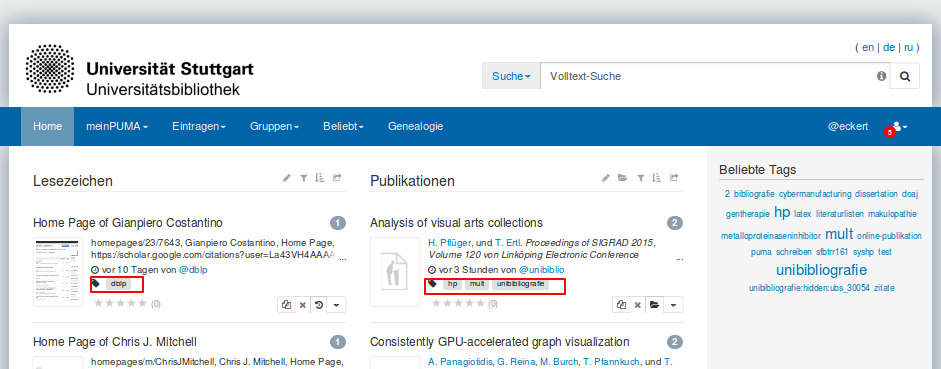
\includegraphics[width=10cm]{Bilder/Kapitel6/Tags}}
 \caption{Tags}
 \label{figure025}
\end{figure}
\textbf{\tags zu Lesezeichen/~Publikationen hinzufügen}\newline
Jeder neue Eintrag braucht mindestens ein \tag. Es können beliebig viele \tags, durch Leerzeichen getrennt, hinzugefügt werden. Beim BiBTeX-Export werden die \tags im Feld \textit{keywords} exportiert.\\
\begin{figure}[h!]
 \centering
 \fbox{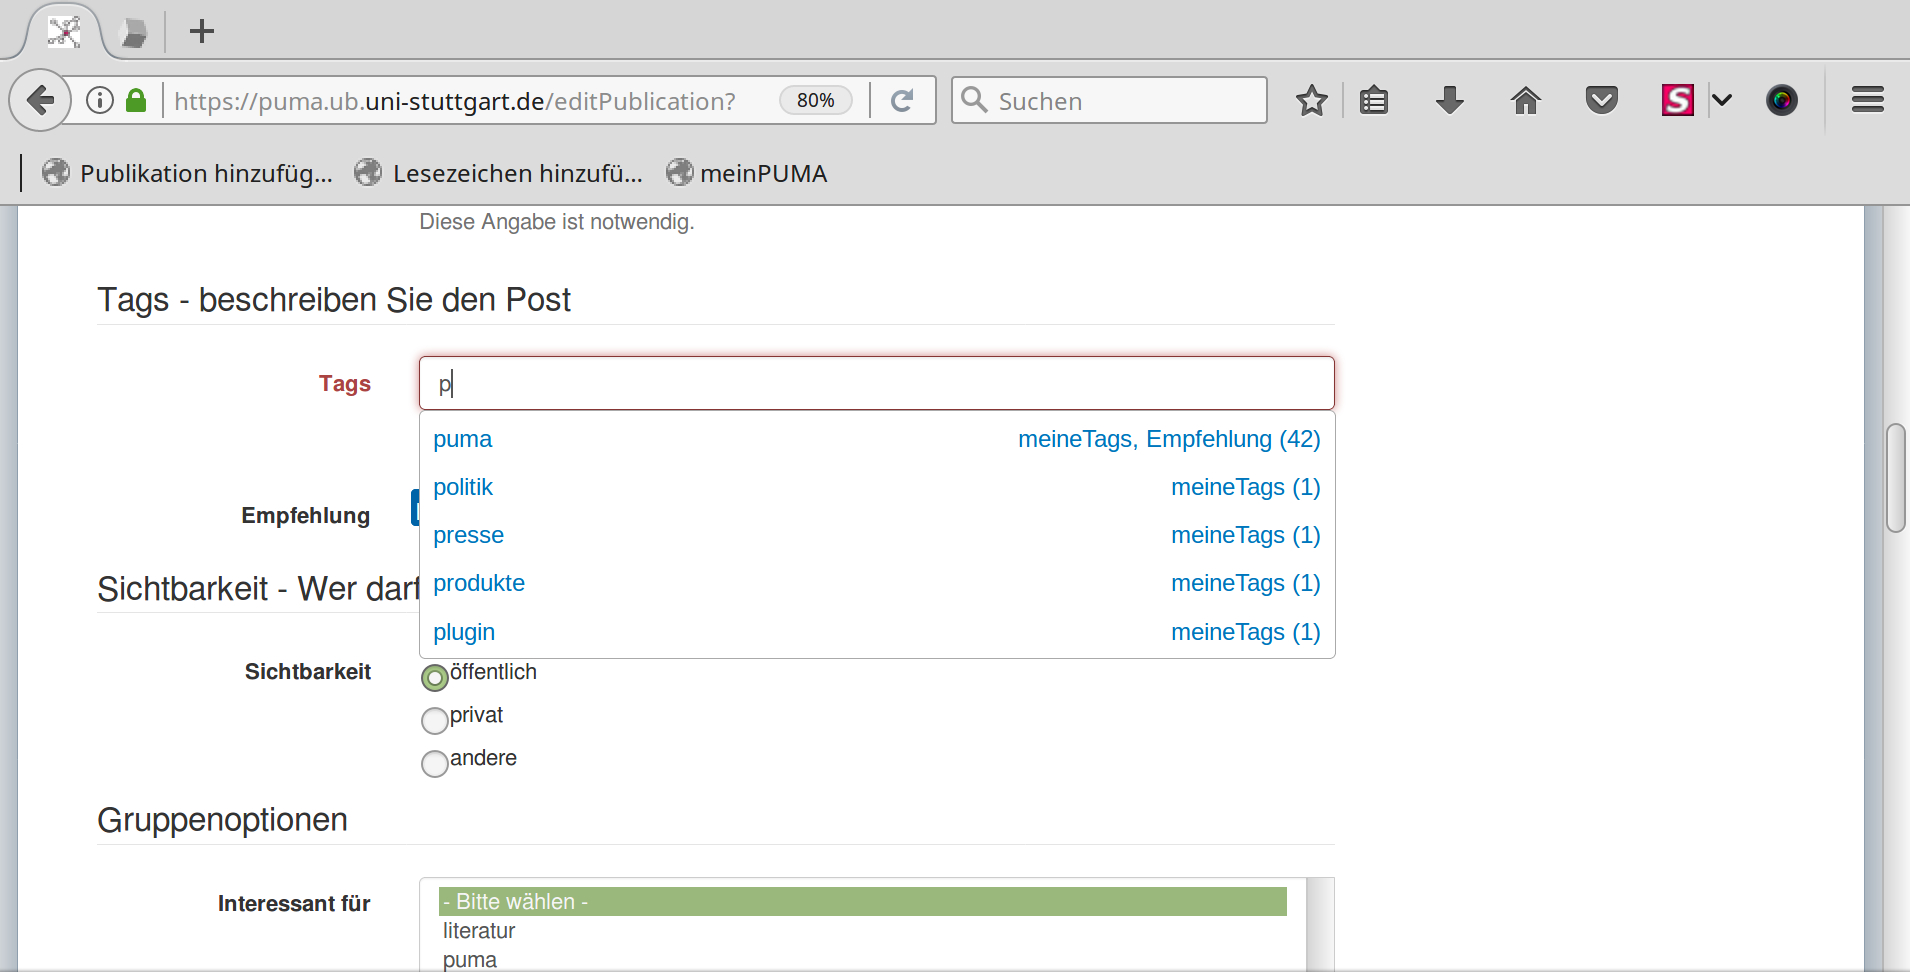
\includegraphics[width=10cm]{Bilder/Kapitel6/Tags_hinzufuegen}}
 \caption{Tags hinzufügen}
 \label{figure026}
\end{figure} 
%\begin{wrapfigure}{l}{7cm}
%\end{wrapfigure}
\textbf{\tags von Lesezeichen/~Publikationen bearbeiten} \newline
PUMA bietet drei Möglichkeit bei Publikationen/~Lesezeichen, die schon Teil einer Sammlung sind, die \tags zu bearbeiten: \index{Tags!bearbeiten}
\begin{itemize}
    \item \underline{\enquote{Schnellbearbeitung}}\newline
   Über das blaue Stiftsymbol (\enquote{\tags bearbeiten}) vor den vorhandenen \tags können diese gelöscht (\enquote{X-Symbol} im blau hinterlegten\tag oder neue hinzugefügt werden. Dazu im Textfeld die \tags durch Leerzeichen getrennt eingeben.
    \item \underline{\enquote{Eintrag bearbeiten}}\newline
    Über die Bearbeitungsfunktion der gesamten Publikation, können auch die \tags angepasst werden. \todo[inline]{Querverweis}
    \item \underline{mehrere \tags bearbeiten}\newline
    PUMA bietet die Möglichkeit alle verwendeten \tags zu bearbeiten. Dazu über das Personensymbol\enquote{Tags bearbeiten} auswählen und eine der folgenden Aktion durchführen:
    \begin{enumerate}
        \item Umbenennen/~Ersetzten von Tags: \newline Hier können \tags ersetzt werden. Z.B. ähnlich geschriebene \tags zu einem \tag zusammenfügen.
    \end{enumerate}
		\begin{tip} Es kann immer nur ein Subtag eingegeben werden, wenn zwei Subtags gleichzeitig eingeben wird das Konzept nicht erstellt. Um mehrere Subtags in einem Konzept zu vereinen, muss der oben genannten Ablauf zur Erstellung eines Konzeptes mit jedem neuen Subtag wiederholt werden.
		\end{tip}
\end{itemize}

\subsection{Systemtags}
\index{Systemtags}
\index{Tags!Systemtags}
\label{subsec:Systemtags}
Systemtags sind spezielle \tags, die eine feste Bedeutung haben.
\begin{enumerate}
    \item \textit{for:<Gruppenname>} : Mit diesem Systemtag wird der Eintrag in die Sammlung der Gruppe kopiert. Der Eintrag ist dann einmal in der eigenen Sammlung und unter dem Benutzer \enquote{Gruppenname} vorhanden. Beim Gruppeneintrag wird der Systemtag durch \textit{from:<Benutzername>} ersetzt. Der Gruppeneintrag ist eine Kopie und ist nicht mehr an den Eintrag aus der eigenen Sammlung gebunden. Nur Mitglieder der Gruppe können Einträge in diese Gruppe kopieren. Gruppenadmins können den Gruppeneintrag editieren.\todo[inline]{alle Infos hier rein? oder wo anders und verweisen}
    \item \textit{send:<Benutzername>} : Damit wird der Eintrag in den Eingang eines befreundeten Benutzers gesendet. Damit dies funktioniert, muss man als Freund beim Empfänger eingetragen oder Mitglied in der gleichen Gruppe sein. Sobald der Eintrag bei dem Nutzer angekommen ist wird der \tag durch \textit{sent:<Benutzername>} ersetzt (vgl. \autoref{sec:Eingang}). \todo{testen} 
Meta-Systemtags sind vom System definiert und erfüllen eine bestimmte Funktion.
    \item \textit{myown:} Durch den \tag wird angegeben, dass man der Verfasser des der Eintrags ist. Ein Eintrag, der mit dem Tag myown\index{myown} versehen wurde, erscheint im Lebenslauf \autoref{MeinProfil}. 
    \item \textit{sys:relevantFor:<Gruppenname>} : Einträge mit dem \tag \textit{sys:relevantFor} werden auf der \enquote{Interessant für\index{Interessant für}}-Seite der Gruppe angezeigt. Damit hat dieser \tag den gleichen Effekt, wie das Auswählen der Gruppe \textit{<Gruppenname>} in der \enquote{Interessant für}-Box beim Bearbeiten eines Eintrages.
    \item \textit{sys:hidden:<tag>} : Mit diesem Systemtag können \tags vor anderen Nutzern versteckt werden. 
\end{enumerate}
\begin{tip}
Das blaue Sternchen vor den \tag-Einträgen symbolisiert die Systemtags. Über dieses Sternchen kann direkt der Systemtag ausgewählt werden und alle Einträge mit diesm \tag werden angezeigt.
\end{tip}

\subsection{Konzepte}
\underline{Was sind Konzepte\index{Konzepte}?\label{subsec:Konzepte}}
\newline
Durch Konzepte können Tags zusammengefasst werden. Beispielsweise sind dem Konzept mit dem Supertag\index{Supertag} (Namen) Obst, die Subtags\index{Subtag} Banane, Apfel und Kiwi zugeordnet. Wenn nun mit dem Konzept Obst gesucht wird, werden alle Publikationen und Lesezeichen angezeigt, die mit mindestens einem der Subtags getagged wurden. 
\newline Die eigenen Konzepte finden sich im Untermenü von \enquote{mein PUMA}. Beliebte Konzepte von allen Nutzern werden unter \enquote{Beliebt} $\to$ \enquote{Konzepte}. 
\newline
\newline
\underline{Konzepte erstellen}
\newline
Konzepte können über das Personensymbol $\to$ \enquote{Tags bearbeiten} erstellt oder überarbeitet werden.
\begin{figure}[h!]
 \centering
 \fbox{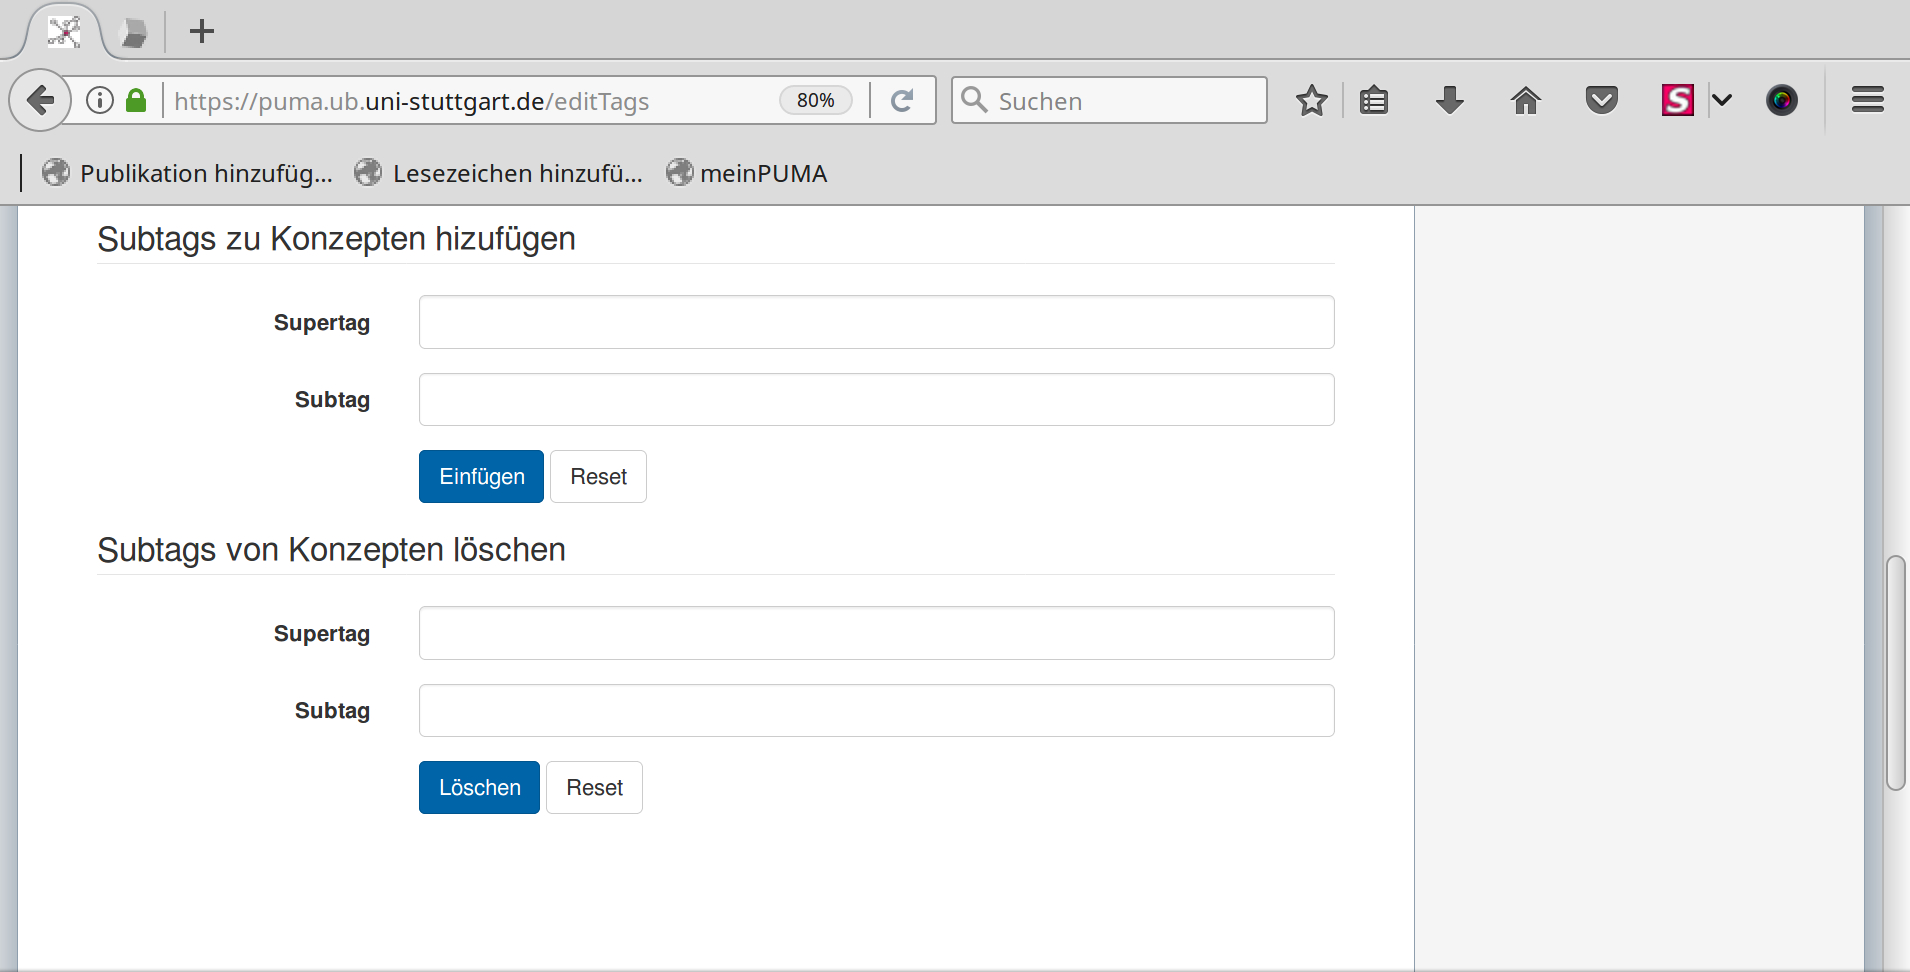
\includegraphics[width=10cm]{Bilder/Kapitel6/Konzepte_erstellen}}
 \caption{Ein Konzept erstellen}
 \label{figure027}
\end{figure}
\textbf{Subtags zu Konzepten hinzufügen:}
Um ein Subtag zu einem Konzept hinzuzufügen, den Namen des Konzepts in das Feld \enquote{Supertag} eingeben und das \tag, das hinzufügt werden soll in das Feld \enquote{Subtag} eintragen. Anschließend auf \enquote{Einfügen} klicken (\autoref{subsec:Konzepte}).
\textbf{Subtags von Konzepten löschen:} Um ein Subtag von einem Konzept zu löschen, den Namen des Konzepts in das Feld \enquote{Supertag} und das zu löschende \tag, in das Feld \enquote{Subtag} eingeben. Anschließend auf \enquote{Löschen} klicken.
\section{Suche}
\label{itm:suchSystemtag}
\textbf{Suchen\index{Suche} \label{Suche} via \tags}\newline
PUMA bietet verschiedene Möglichkeiten, mit Hilfe der \tags Lesezeichen und Publikationen zu finden: \\
\begin{itemize}
\item Um einen Eintrag mit einem bestimmten \tag zu finden, in der Suchleiste neben \enquote{Suche} auf den blauen Pfeil klicken und im Dropdown-Menü \enquote{\tag} auswählen. \\
\item Wenn ein \tag bei einem Eintrag angeklickt wird, öffnet sich eine Seite mit allen Einträgen des Nutzer mit diesem bestimmten \tag. Auf der rechten Seite finden sich weitere Informationen zu diesem \tag: Unter \enquote{Stöbern} wird angezeigt wie oft dieser \tag von allen Nutzern verwendet wurde. Unter verwandten \tags werden \tags angezeigt, die zusammen mit dem ausgewähltem \tag verwendet wurden. Darüber hinaus werden die Konzepte \autoref{subsec:Konzepte} und die verwendeten \tags des Nutzers.\\
\end{itemize}
Such-Systemtags können Einträge nach Suchanfragen filtern. Alle Such-Systemtags haben die gleiche Syntax: \textit{sys:<Feldname>:<Feldwert>}. Beispielsweise werden  bei der Suchanfrage \textit{sys:author:panther} nur die Einträge angezeigt, welche von dem Autor \textit{Panther} stammen.\newline
Die Syntax kann entweder in die Suchleiste oder mit der URL eingeben werden. Folgende Filter unterstützt PUMA (Suche beschränkt sich auf die Publikationseinträge):\newline
\newline
Für die Suche nach einem bestimmten Autor oder Erscheinungsjahr muss vorher festgelegt werden, in welchen Einträgen eines Nutzers nach dem Autor oder dem Erscheinungsjahr gesucht werden soll. Zum Beispiel sucht: \newline https://puma.ub.uni-stuttgart.de/user/panther/sys:year:2013 \newline Publikationen aus dem Jahr 2013 in den Einträgen des Nutzers Panther. 
\begin{enumerate}
    \item \textit{sys:author:<Autorenname>} filtert die Suche nach dem Autor.
		\item \textit{sys:not:<tag>} filtert die Suche, indem alle Ergebnisse ignoriert werden, die diesen Tag enthalten. An dieser Stelle können auch Platzhalter verwendet werden, z.B. werden bei sys:not:news\_ 
    alle Ergebnisse ignoriert, die Tags enthalten, die mit news\_
    beginnen.
    \item \textit{sys:year:<Jahr>} filtert die Suche nach dem Erscheinungsjahr. Dabei sind mehrere Schreibweisen für das Jahr möglich:
    \begin{enumerate}
        \item 2000: Alle Einträge aus dem Jahr 2000
        \item 2000-: Alle Einträge aus dem Jahr 2000 oder einem Jahr danach
        \item -2000: Alle Einträge aus dem Jahr 2000 oder einem Jahr davor
        \item 1990-2000: Alle Einträge aus den Jahren 1990 bis 2000
    \end{enumerate}
%muss noch raus rutschen
Bei der Suche nach Titel, Gruppe, Nutzer, usw. spielt der Nutzer keine Rolle. Es muss nur der Zusatz tag/ vor die Suchsyntax gesetzt werden, zum Beispiel  https://puma.ub.uni-stuttgart.de/tag/sys:entrytype:article. Damit finden sich alle Artikel, die auf PUMA eingetragen wurden.
    \item \textit{title:<title>} sucht nach Einträgen mit diesem Titel.
    \item \textit{user:<user>} sucht nach Einträgen eines Nutzers.
    \item \textit{group:<group>} filtert die Suche nach einer bestimmten Gruppe.
    \item \textit{entrytype:<Eintragstyp>} filtert die Suche nach dem Eintragstypen. Eintragstypen\footnote{\url{https://www.ctan.org/pkg/biblatex?lang=de}} werden verwendet, um BibTex-Einträge nach ihren Typen zu klassifizieren. Derzeit unterstützt Puma folgende Eintragstypen\index{Eintragstypen}: 
    \begin{enumerate}
        \item \textbf{article\index{Article}:} Zeitungs- oder Zeitschriftenartikel\newline
        Erforderliche Felder: Autor, Titel, Zeitschriftentitel, Ausgabennummer, Jahr/Datum 
        \item \textbf{book\index{Book}:} Buch, Monografie mit angegebenem Verlag\newline
        Erforderliche Felder: Autor, Titel, Jahr
        \item \textbf{booklet\index{Booklet}:} Gebundenes Druckwerk, aber ohne Verlag oder Sponsororganisation\newline
        Erforderliche Felder: Autor/Lektor, Titel, Jahr/Datum
        \item \textbf{conference\index{Conference}:} Ein Beitrag zu einer Konferenz, der nicht in einem Konferenzband erschienen ist\newline
        Erforderliche Felder: Autor, Titel, Buchtitel, Jahr/Datum
        \item \textbf{electronic\index{Electronic}:} Elektronische Veröffentlichungen, z. B. eBooks oder Blogeinträge\newline 
        Erforderliche Felder: Autor, Buchtitel, Verlag, Adresse, Jahr
        \item \textbf{inbook\index{Inbook}:} Teil eines Buches, z. B. ein Kapitel oder ein Seitenbereich\newline
        Erforderliche Felder: Autor, Titel, Buchtitel, Jahr/Datum 
        \item \textbf{incollection\index{Incollection}:} Teil eines Buches mit einem eigenem Titel, z. B. Beitrag in einem Sammelband\newline
        Erforderliche Felder: Autor, Titel, Buchtitel, Jahr/Datum
        \item \textbf{inproceedings\index{Inproceedings}:} Artikel in einem Tagungsband bzw. Konferenzband\newline
        Erforderliche Felder: Autor, Titel, Buchtitel, Jahr/Datum
        \item \textbf{manual\index{Manual}:} Technische Dokumentation, Handbuch\newline
        Erforderliche Felder: Autor/Lektor, Titel, Jahr/Datum
        \item \textbf{mastersthesis\index{Mastersthesis}:} Master-, Magister- oder Diplomarbeit\newline
        Erforderliche Felder: Autor, Titel, Art der Arbeit, Institut, Jahr/Datum
        \item \textbf{misc\index{Misc}:} Diesen Eintragstyp können Sie wählen, wenn nichts anderes zu passen scheint. \newline
        Erforderliche Felder: Autor/Lektor, Titel, Jahr/Datum
        \item \textbf{patent\index{Patent}:} Patent\newline 
        Erforderliche Felder: Autor, Titel, Nummer, Jahr/Datum
        \item \textbf{periodical\index{Periodical}:} Ein regelmäßig erscheinendes Werk, z.B. Zeitschrift\newline
        Erforderliche Felder: Lektor, Titel, Jahr/Datum
        \item \textbf{phdthesis\index{Phdthesis}:} Doktor- oder andere Promotionsarbeit\newline 
        Erforderliche Felder: Autor, Titel, Hochschule/Universität, Jahr 
        \item \textbf{presentation\index{Presentation}:} Präsentation, Vortrag auf einer Veranstaltung\newline 
        Erforderliche Felder: Verfasser, Titel, Anlass der Präsentation, Jahr
        \item \textbf{proceedings\index{Proceedings}:} Tagungsband einer Konferenz\newline
        Erforderliche Felder: Titel, Jahr/Datum
        \item \textbf{standard\index{Standard}:} Standard\newline 
        Erforderliche Felder: Autor, Buchtitel, Verlag, Adresse, Jahr 
        \item \textbf{techreport\index{Techreport}:} Bericht einer Hochschule oder einer anderen Institution\newline
        Erforderliche Felder: Autor, Titel, Jahr/Datum
        \item \textbf{unpublished\index{Unpublished}:} Nicht formell veröffentlichtes Dokument\newline 
        Erforderliche Felder: Autor, Titel, Jahr/Datum
    \end{enumerate}
    \item \textit{bibtexkey:<bibtexkey>} filtert die Suche nach einem bestimmten BibTeX-Schlüssel.
\end{enumerate}
\subsection{Publikationen durchstöbern}
Um sich schnell einen Überblick über die eigenen Einträge machen zu können, bietet PUMA die Funktion \enquote{Publikation\index{Publikationen!durchstöbern} durchstöbern} an. Über \enquote{meinPUMA} \enquote{Publikationen durchstöbern} auswählen. Unter \enquote{Suchoptionen} können die Publikationen nach \tags und Autoren durchsucht werden. Mit \enquote{und/~oder} kann die Art der Suche bestimmt werden. Das Textfeld \enquote{Filter} ermöglicht es die Suchbegriffe direkt einzugebn oder die Ergebnisse noch weiter zu filtern.
\begin{figure}[h!] 
\centering
 \fbox{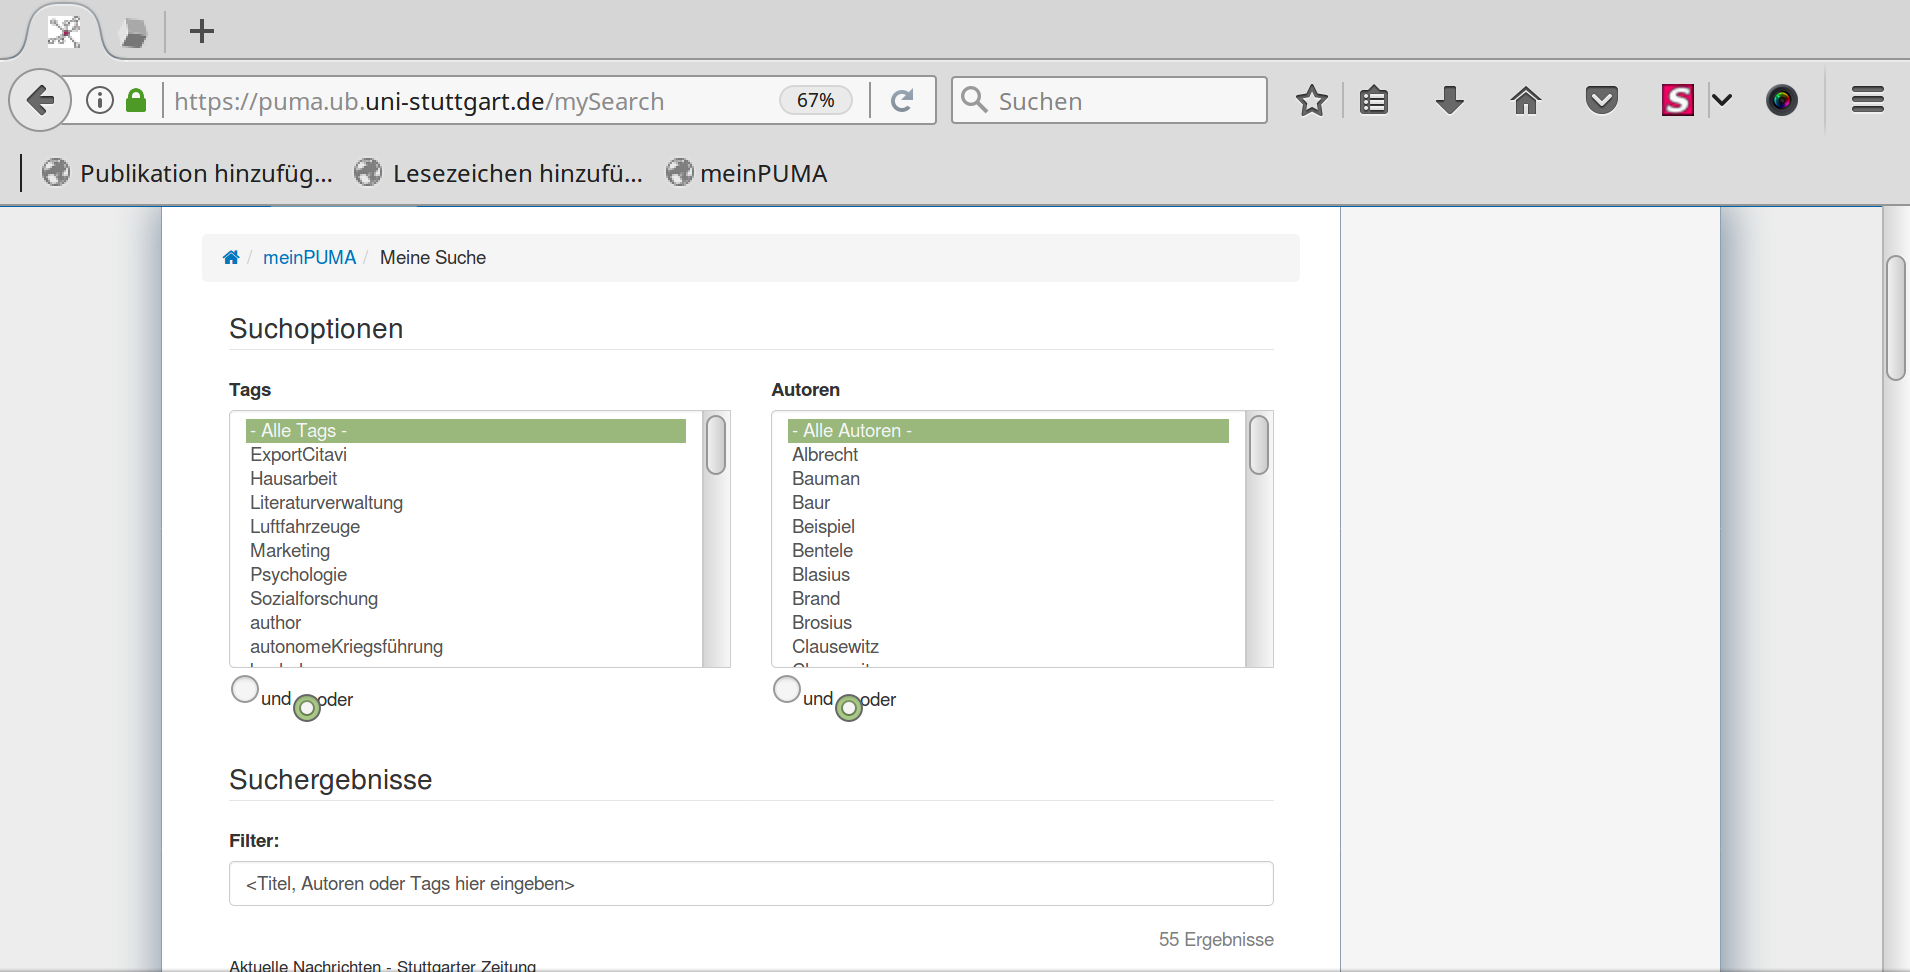
\includegraphics[width=10cm]{Bilder/Kapitel6/Publikationen_durchstoebern}}
 \caption{Publikationen durchstöbern}
 \label{figure029}
\end{figure}
\section{Duplikate}
PUMA legt für jede Sammlung einen eigenen Eintrag an. Es kann also vorkommen, dass ein Eintrag mehrmals bei verschiedenen Nutzern in der Sammlung eingetragen wird. Wie oft dieser Eintrag vorhanden ist, ist an der Zahl oben rechts neben dem Eintrag erkennbar. Wenn Publikationen aus einer Gruppe exportiert werden sollen, besteht die Möglichkeit über den Befehl \enquote{\textit{dublicates=no}} zu verhindern, dass ein Eintrag mehrmals auftaucht. \todo[inline]{wie werden Dubletten in der Ausgabe unterdrückt? Verweis auf ausführlichere Anleitung?}
Beim Sammeln von Publikationen kann es vorkommen, dass diese zweimal in die eigene PUMA-Sammlung eingetragen werden. Hier bietet PUMA die Möglichkeit Duplikate\index{Duplikate} in der eigenen Sammlung zu erkennen. Um zu sehen, ob Duplikate in der eigenen Sammlung existieren, über das Dropdownmenü bei \enquote{meinPuma} \enquote{Duplikate} auswählen. Hier kann dann ein Eintrag gelöscht werden.
Manchmal besteht auch das umgekehrte Problem, wenn ein ähnlicher Eintrag aufgenommen werden soll und nur der bestehende geändert werden kann. Dies kann umgegangen werden, indem entweder das Feld \enquote{Volume} oder \enquote{number} anders belegt wird.(Zur Erklärung: \autoref{sec:duplikat})
\begin{figure}[h!]
 \centering
 \fbox{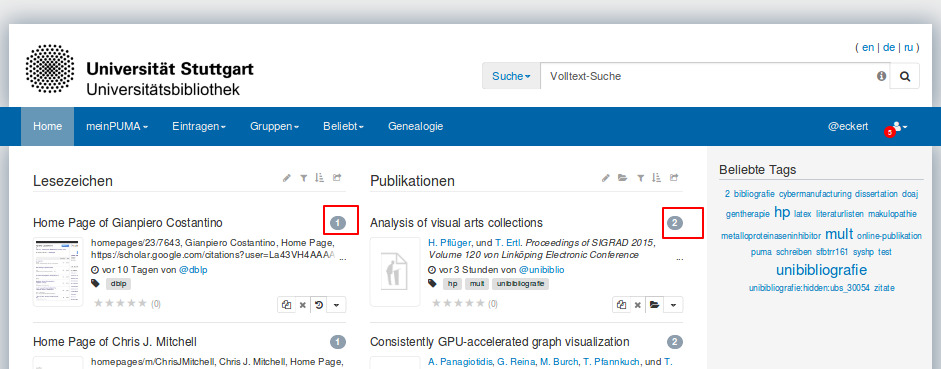
\includegraphics[width=10cm]{Bilder/Kapitel6/Duplikate}}
 \caption{Duplikate}
 \label{figure027}
\end{figure}
\section{Private Dateien anhängen}
An jeden Publikationseintrag kann beim Eintragen der Metadaten ein Dokument\index{Dokumente! anhängen} angehängt werden (max. 50 MB pro Datei - erlaubte Dateiendungen: pdf, ps, djv, djvu, txt, tex, doc, docx, ppt, pptx, xls, xlsx, ods, odt, odp, jpg, jpeg, svg, tif, tiff, png, htm, html, epub). Der Anhang ist aus urheberrechtlichen Gründen nur in der eigenen Sammlung, für Freunde und in einer gemeinsamen Gruppe sichtbar.
Wenn die angehängte Datei auch für Gruppenmitglieder sichtbar sein soll, muss der Gruppenadministrator das Teilen von Dokumenten erlauben
und die einzelnen Mitglieder dies ebenfalls in ihrer Gruppeneinstellung freischalten. In den Einstellungen kann der Nutzer unter dem Reiter \enquote{Gruppen} für jede einzelne Gruppe festlegen, ob Dateien geteilt werden oder nicht. Diese Funktion kann jederzeit wieder deaktiviert werden.
\begin{figure}[h!]
 \centering
 \fbox{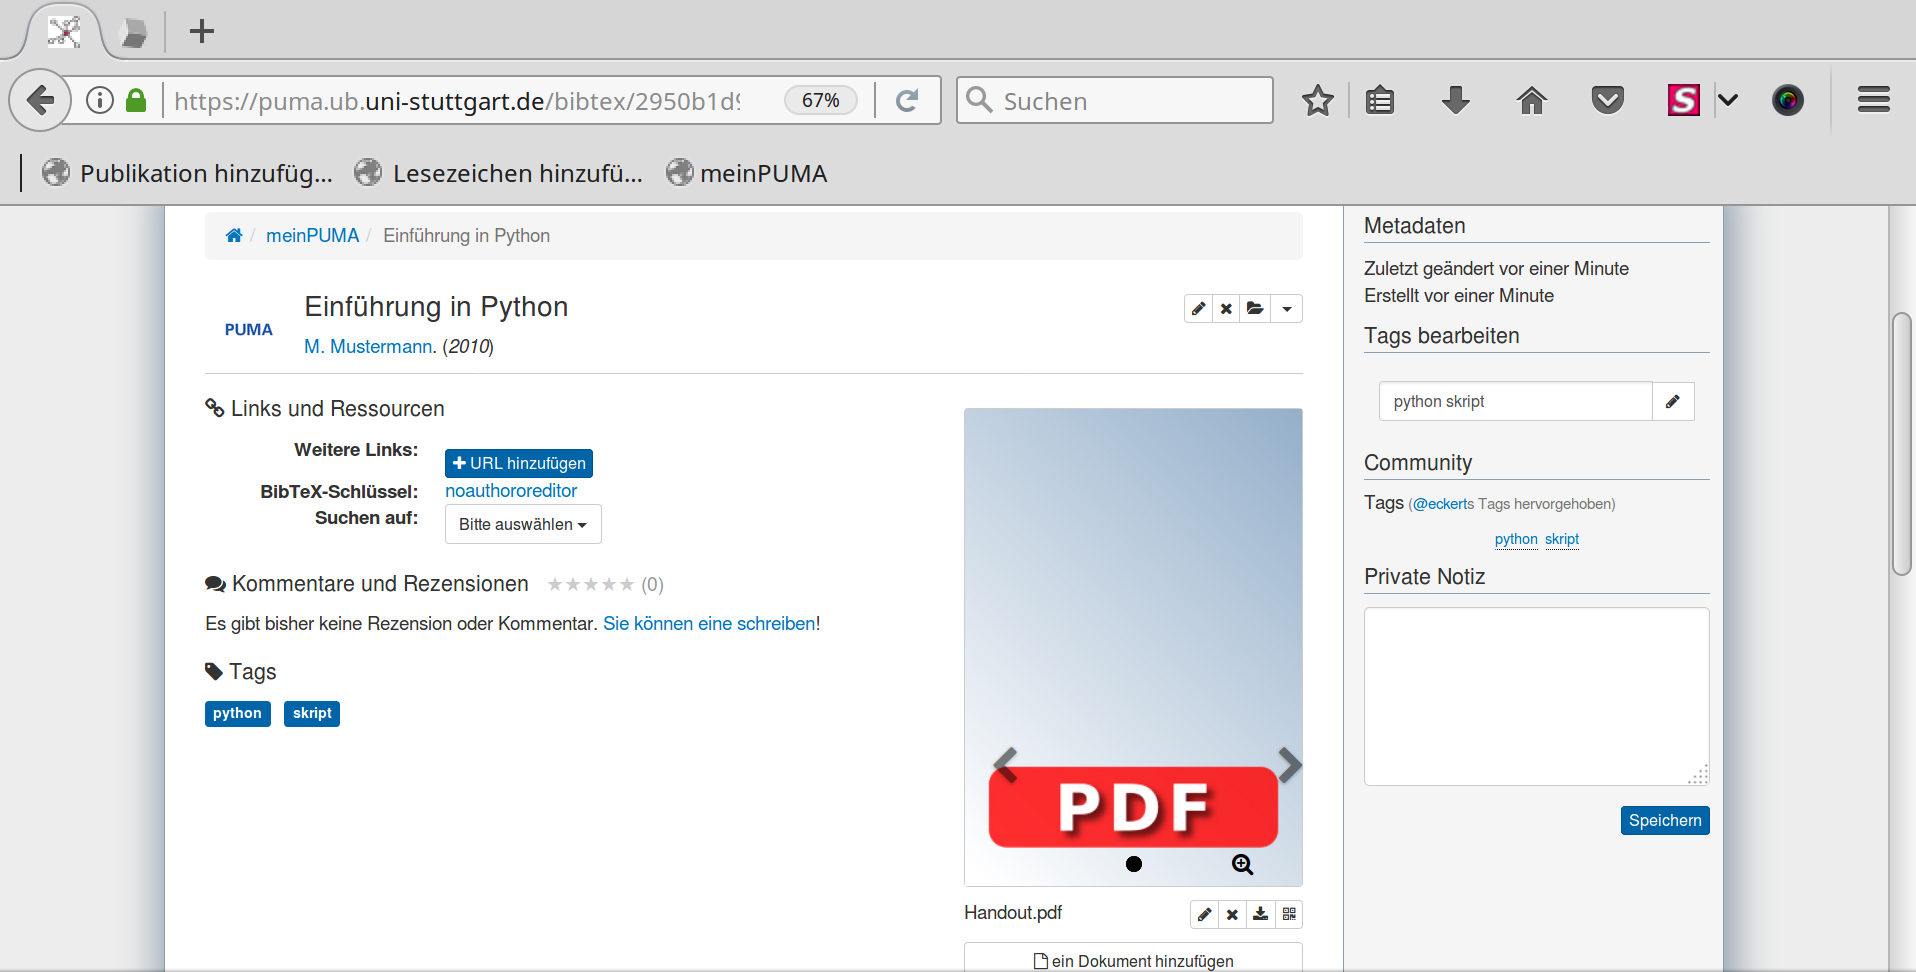
\includegraphics[width=10cm]{Bilder/Kapitel6/Private_Dokumente}}
 \caption{Private Dokumente anhängen}
 \label{figure028}
\end{figure}

\section{Zugriff auf Publikationen erhalten}
\label{subsec:OpenURL}
In PUMA existieren verschiedene Möglichkeiten an die Publikationen hinter den bibliografischen Einträgen zu gelangen. 
\subsection{DOI und OpenURL}
Unter jeder Publikation befindet sich ganz rechts ein schwarzer Pfeil, über ein Dropdownmenü, kann einerseits die Publikation in ein gewünschtes Format (vgl.\autoref{sec:EExpo}) exportiert werden. Andererseits besteht die Möglichkeit direkt auf die Publikation zu gelangen. Wenn eine DOI oder eine URL vom Nutzer hinterlegt wurde, sind die entsprechenden Felder schwarz hinterlegt und können angeklickt werden. Wenn die Unibibliothek die entsprechende Zeitschrift oder das E-Book lizenziert hat, ist normalerweise auch der Volltext (wenn man sich im Uninetz befindet) verfügbar. Wenn nicht oder wenn die Publikation nur in print vorliegt, kann über \enquote{Standard OpenURL-Server} direkt im Bibliothekskatalog nach der Publikation gesucht werden. Auch andere Kataloge können über OpenUrl angebunden werden. Dazu die entsprechende Open-URL, in die Einstellungen bei \enquote{Mein Profil} (vgl. \autoref{MeinProfil} kopieren. Über \enquote{Ihr OpenURL-Server} ist nun auch die Suche in dem ausgewählten Katalog möglich.
%\url{http://www.redi-bw.de/links/unist} 

\begin{figure}[h!]
 \centering
 \fbox{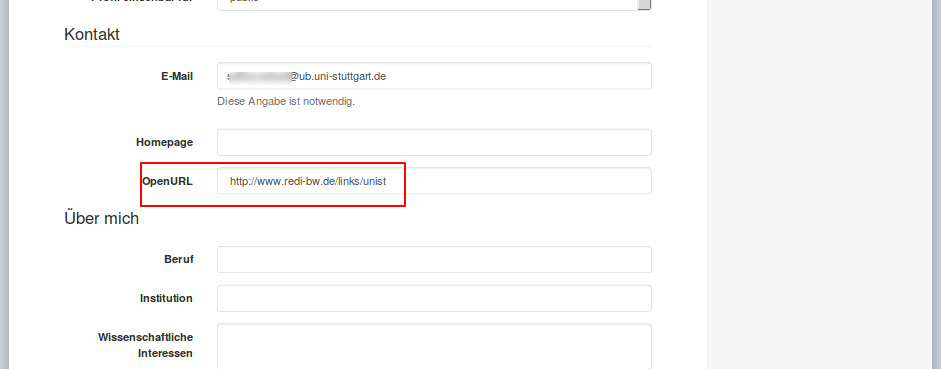
\includegraphics[width=10cm]{Bilder/Kapitel6/Open_URL}}
 \caption{Open-URL der Universität Stuttgart}
 \label{figure031}
\end{figure}


\begin{figure}[h!]
 \centering
 \fbox{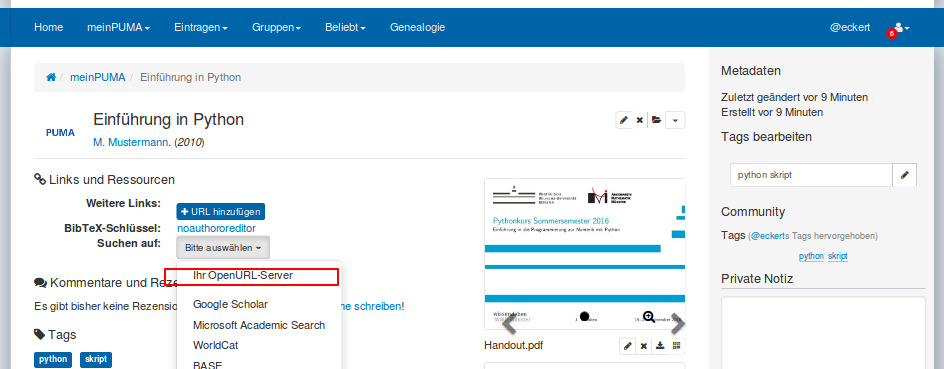
\includegraphics[width=10cm]{Bilder/Kapitel6/OpenURL-Resolver}}
 \caption{OpenURL-Resolver}
 \label{figure032}
\end{figure}
\subsection{Weitere Möglichkeiten Publikationen im Netz zu suchen}%Screenshot
Über die Detailansicht einer Publikation gibt es weitere Möglichkeiten nach dem Volltext einer Publikation zu suchen. Die Detailansicht öffnet sich über den Titel einer Publikation. Das Auswahlmenü \enquote{Suchen auf} bietet die Möglichkeit wieder über die oben erwähnten OpenURL-Server zu suchen. Darüber hinaus kann direkt in Google Scholar, Microsoft Bing, WorldCat und BASE nach der Publikation gesucht werden..

\begin{figure}[h!]
 \centering
 \fbox{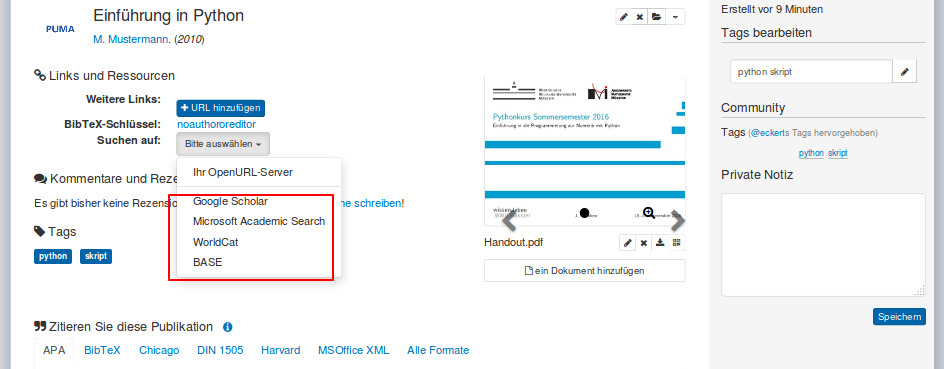
\includegraphics[width=10cm]{Bilder/Kapitel6/Open-Access}}
 \caption{Open Access}
 \label{figure033}
\end{figure}

\section{Eingang}
\label{sec:Eingang}
Im Eingang\index{Eingang} befinden Sie alle Beträge, die von Freunden (vgl. \autoref{sec:freunde}) geschickt wurden.
\begin{figure}[h!]
 \centering
 \fbox{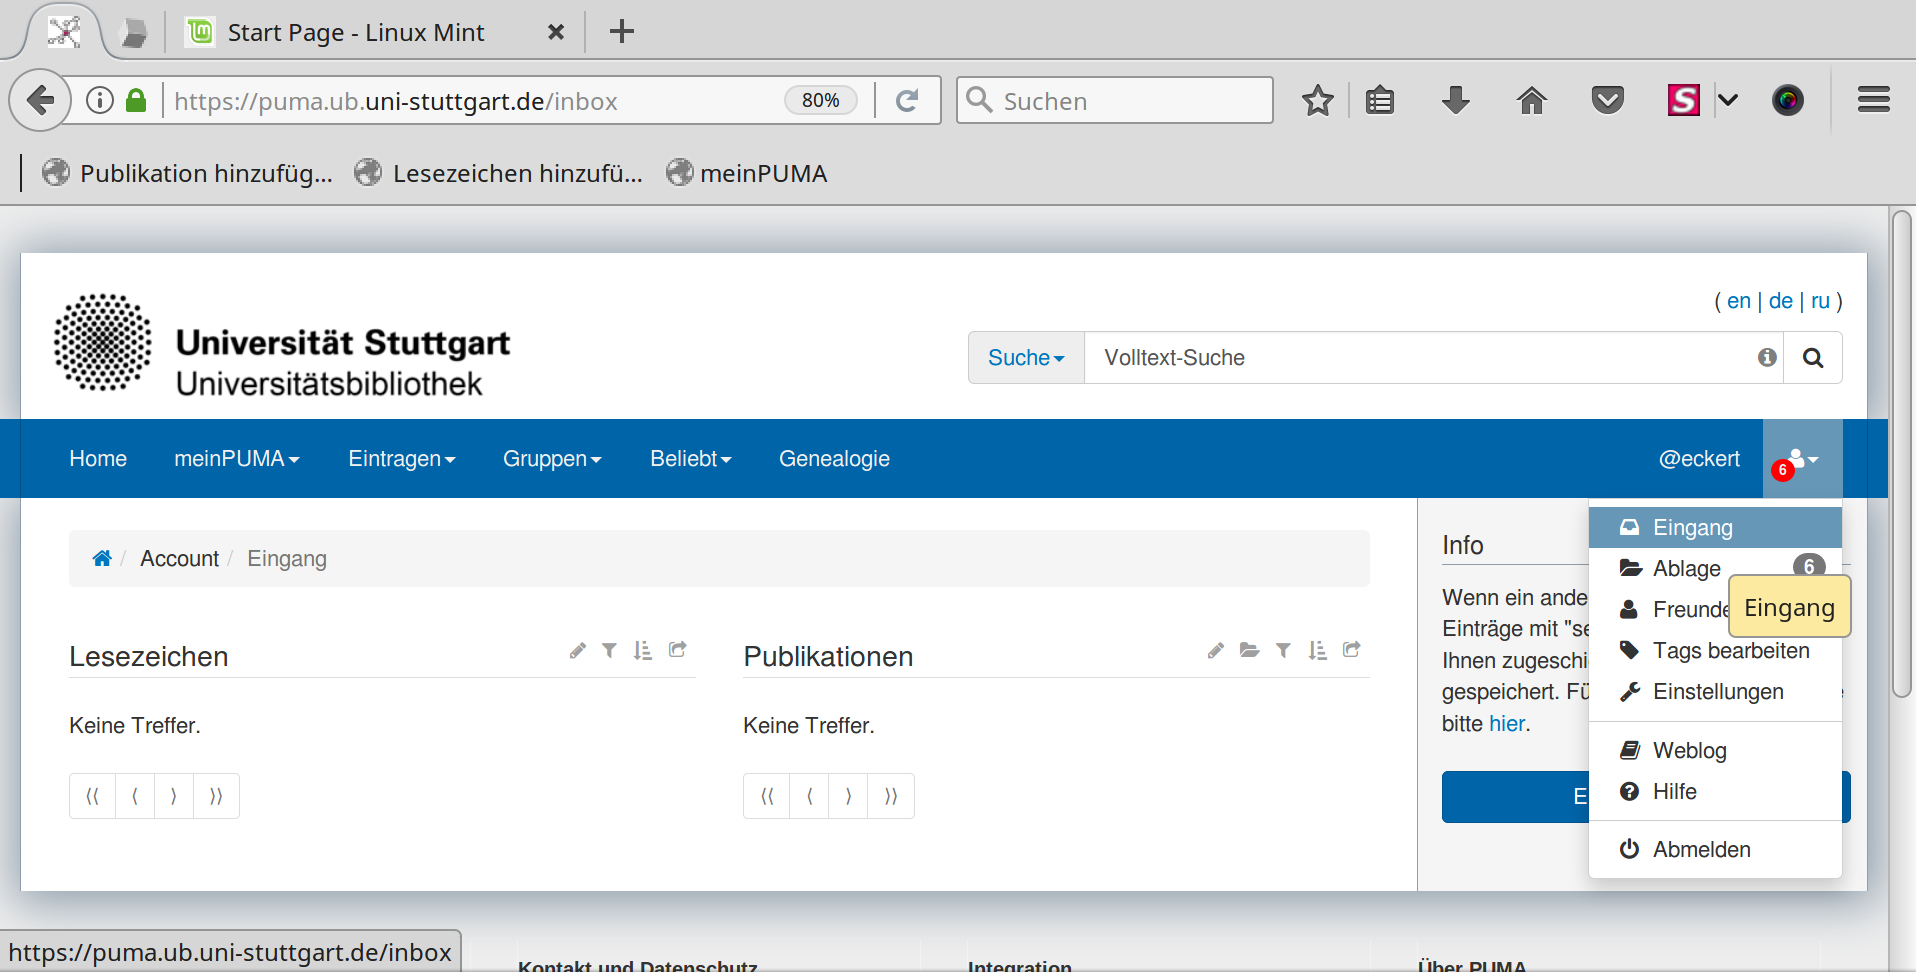
\includegraphics[width=10cm]{Bilder/Kapitel6/Eingang}}
 \caption{Der Eingang}
 \label{figure034}
\end{figure}

\subsection{Einträge verschicken}
\index{Einträge!verschicken}
Einem befreundeten Nutzer kann ein Lesezeichen oder eine Publikation über das Systemtag \textit{send:Nutzername}geschickt werden 
(vgl. \autoref{subsec:Systemtags}). Diesen \tag beim Eintragen einer Publikation/Lesezeichen mit eingeben. Der Eintrag wird dann mit from:<eigenerNutzername> getaggt und in den Eingang des anderen Nutzers kopiert. Um den Missbrauch des Eingangs zu verhindern, muss der Empfänger des Eintrags
\begin{itemize}
    \item entweder mit Ihnen befreundet sein
    \item oder Mitglied einer gemeinsamen Gruppe sein.
\end{itemize}
Nachdem der Eintrag gesendet wurde wird der Tag automatisch von \textit{send:Nutzername} in \textit{sent:Nutzername}  umgewandelt.

\subsection{Einträge erhalten}
\index{Einträge!erhalten}
Im Eingang liegen alle Einträge, die einem geschickt wurden. Diese Einträge können über den Doppelblatt-Button \enquote{Diese Publikation in die eigene Sammlung einfügen}, rechts unter dem Eintrag übernommen werden. Mit dem Kreuz-Symbol \enquote{Diese Publikation aus Ihrem Eingang entfernen}kann der Eintrag aus dem Eingang gelöscht werden. Über \enquote{Eingang leeren} in der rechten Menüleiste, kann der ganze Eingang geleert werden.

%\section{Literaturlisten erstellen}
%PUMA bietet die Möglichkeit, aus den gesammelten Publikationen Literaturlisten\index{Literaturlisten} zu erstellen, die später beispielsweise auf externen Webseiten eingebunden werden können. \newline
%Hierfür fügen Sie die Publikationen, die in das Literaturverzeichnis sollen, zu Ihrer Ablage\index{Ablage} hinzu. Wenn Sie alle Publikationen hinzugefügt haben, klicken Sie in der Ablage, oberhalb von den Publikationen, auf Exportzeichen und wählen Sie \enquote{mehr...} aus. Sie gelangen nun zu einer Übersichtsseite, auf der Ihnen alle verfügbaren Zitationsstile angezeigt werden, und Sie nur noch den passenden aussuchen müssen. 
%\subsection{Eigene Literaturlisten erstellen} 
%Neben den Layouts für das Erstellen einer Literaturliste können Sie auch folgenden URLs verwenden, die Sie in Ihren Browser eingeben:
%\begin{enumerate}%Beispielscreenshots ?
    %\item \textbf{Allgemeine Liste:}\newline
    %\textit{https://puma.ub.uni-stuttgart.de/publ/user/<username>} \newline
    %Ersetzen Sie \textit{<username>} durch Ihren Benutzernamen und Ihnen werden alle Publikationen aus Ihrer Sammlung in einer Literaturliste angezeigt.\newline
    %\textbf{Beispiel:} https://puma.ub.uni-stuttgart.de/publ/user/eckert 
%\begin{figure}[h!]
 %\centering
 %\fbox{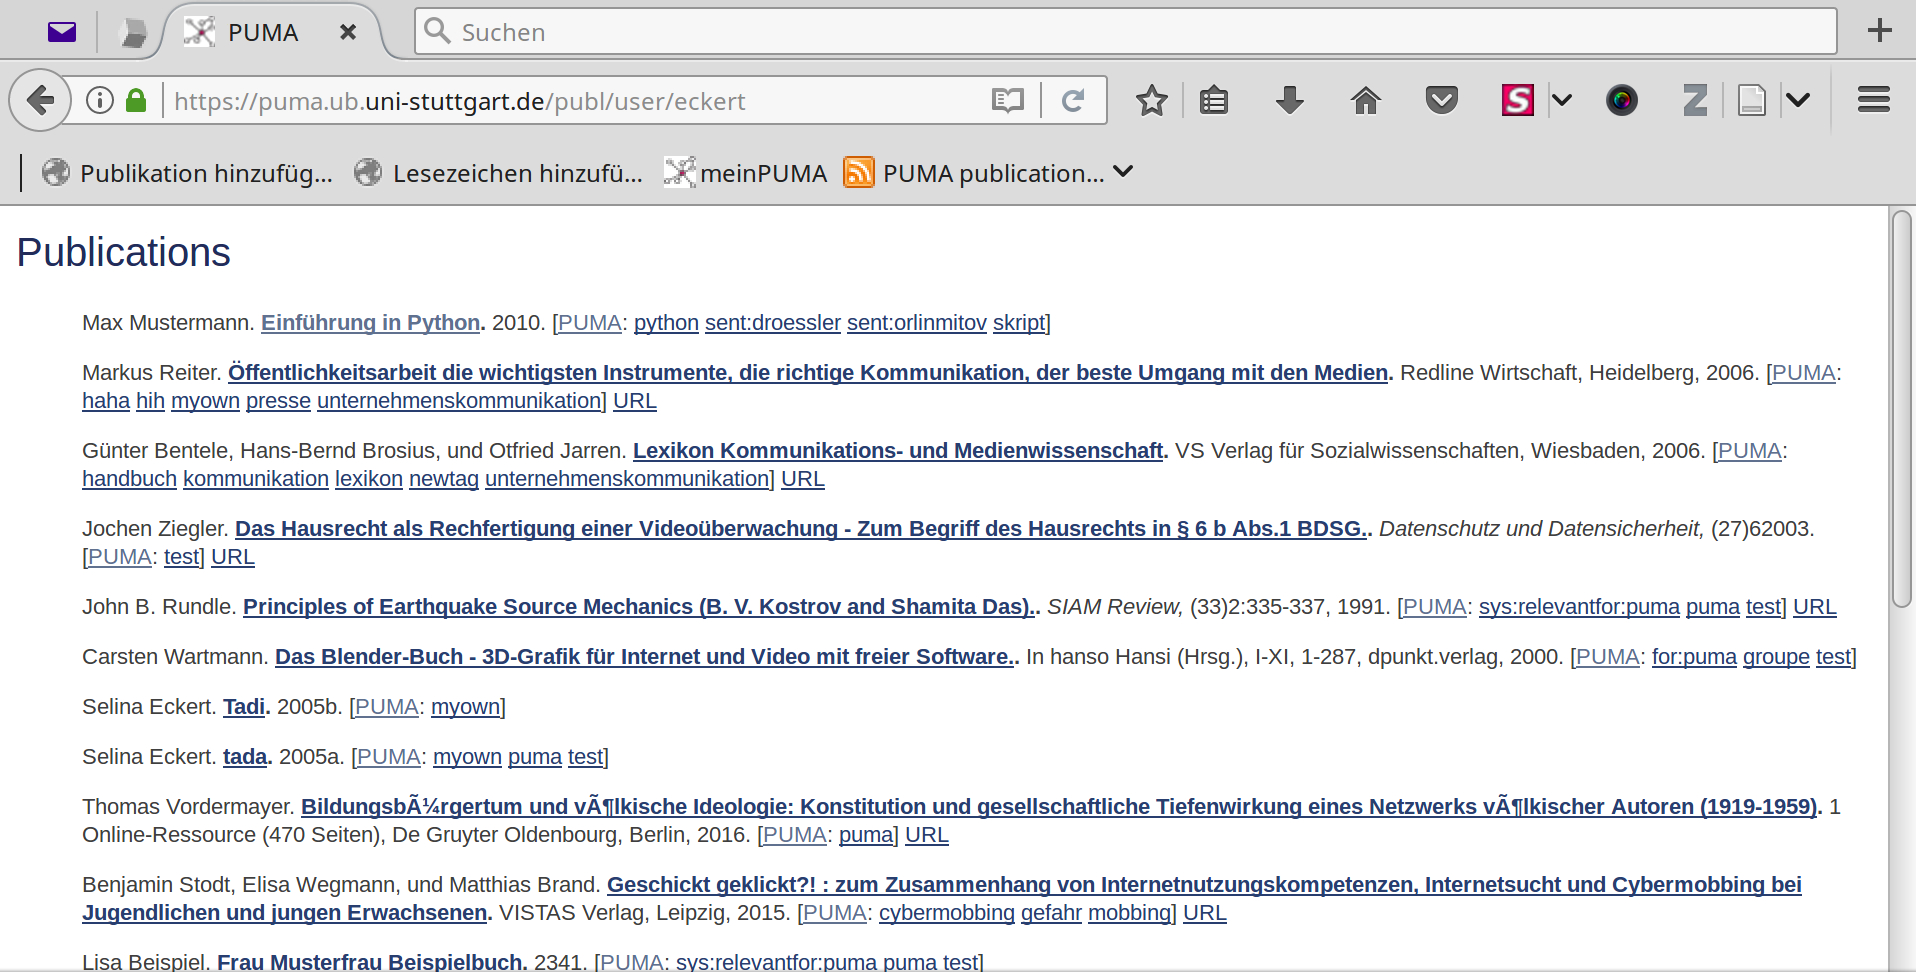
\includegraphics[width=11cm]{Bilder/Kapitel6/Allgemeine_Liste}}
 %\caption{Allgemeine Liste}
 %\label{figure035}
%\end{figure}
%
    %\item \textbf{Allgemeine Liste ohne Tags:}\newline
    %\textit{https://puma.ub.uni-stuttgart.de/publ/user/<username>?notags=1}\newline
    %Ersetzen Sie \textit{<username>} durch Ihren Benutzernamen und Ihnen werden alle Publikationen aus Ihrer Sammlung, ohne Tags, in einer Literaturliste angezeigt.\newline
    %\textbf{Beispiel:} https://puma.ub.uni-stuttgart.de/publ/user/eckert?notags=1 
    %
%\begin{figure}[h!]
 %\centering
 %\fbox{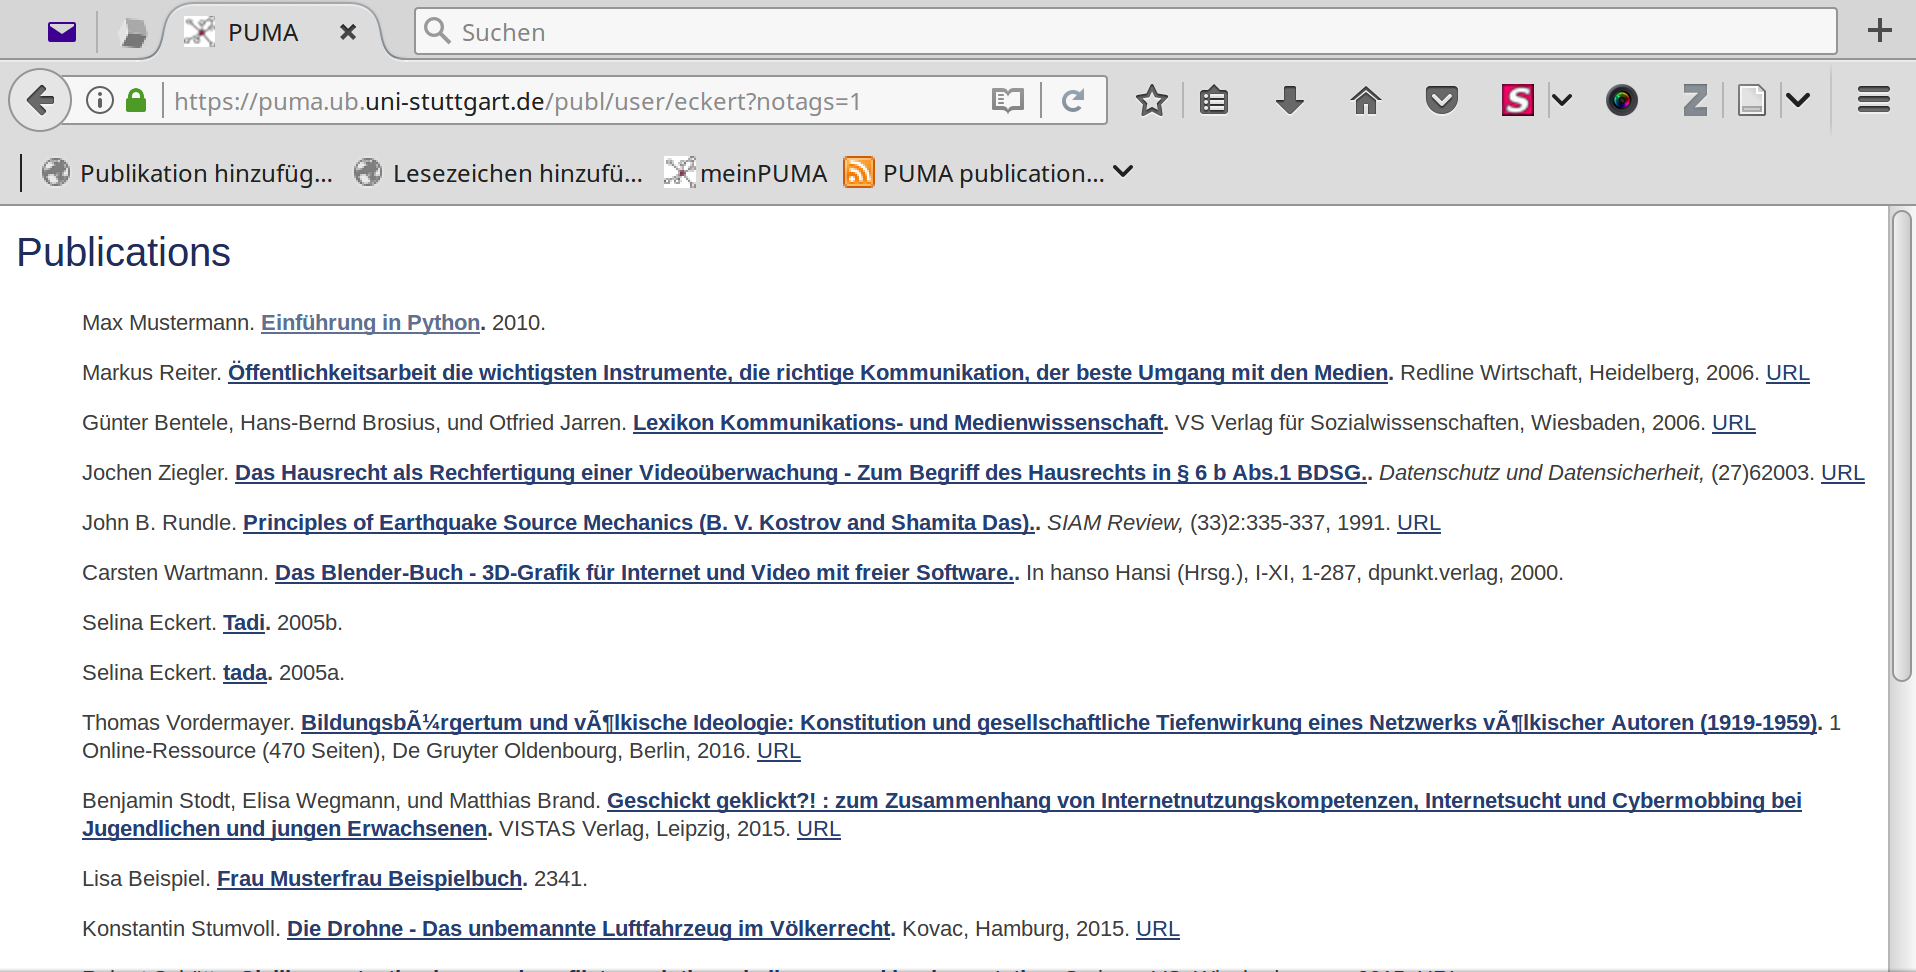
\includegraphics[width=11cm]{Bilder/Kapitel6/Allgemeine_Liste_ohne_Tags}}
 %\caption{Allgemeine Liste ohne Tags}
 %\label{figure036}
%\end{figure}
%
    %\item \textbf{Allgemeine Liste mit Tag-Einschränkung:}\newline
    %\textit{https://puma.ub.uni-stuttgart.de/publ/user/<username>/<tagname>}\newline
    %Ersetzen Sie \textit{<username>} durch Ihren Benutzernamen und \textit{<tagname>} durch den Tag, der in den Publikationen enthalten sein soll. Ihnen wird eine Literaturliste angezeigt, die jene Publikationen aus Ihrer Sammlung enthält, die den speziellen Tag enthalten. Ein besonderes Beispiel hierfür ist der Tag \textit{myown\index{myown}}. Durch diesen Tag geben Sie an, dass Sie der/~die Verfasser/~in der Publikation sind. \newline
    %\textbf{Beispiel:} https://puma.ub.uni-stuttgart.de/publ/user/eckert/puma
   %
%\begin{figure}[h!]
 %\centering
 %\fbox{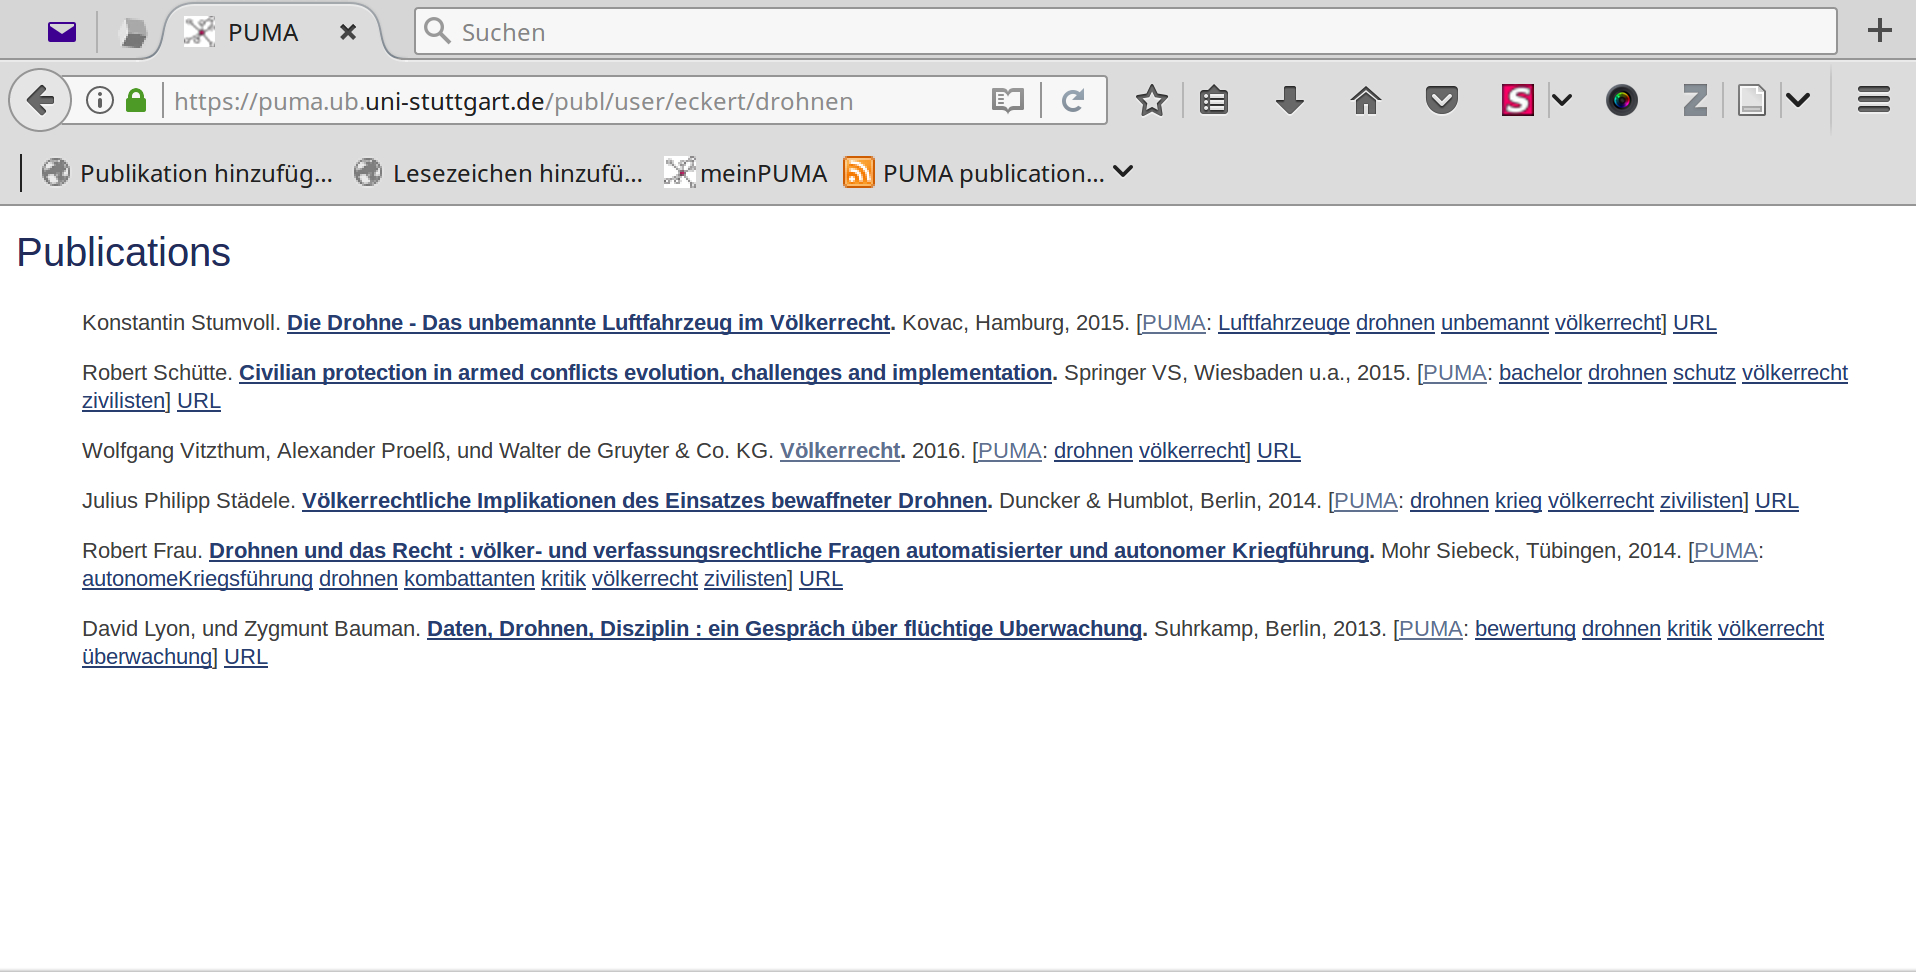
\includegraphics[width=11cm]{Bilder/Kapitel6/Allgemeine_Liste_Tag_Einschraenkung}}
 %\caption{Liste mit Tagauswahl}
 %\label{figure037}
%\end{figure}
%
    %\item \textbf{BibTeX-Liste:}\newline
    %\textit{https://puma.ub.uni-stuttgart.de/bib/user/<username>} \newline
    %Ersetzen Sie \textit{<username>} durch Ihren Benutzernamen. Ihnen wird eine Literaturliste mit all Ihren Publikationen im BibTex-Format\index{BibTex} angezeigt.\newline
    %\textbf{Beispiel:} https://puma.ub.uni-stuttgart.de/bib/user/eckert 
%
%\begin{figure}[h!]
 %\centering
 %\fbox{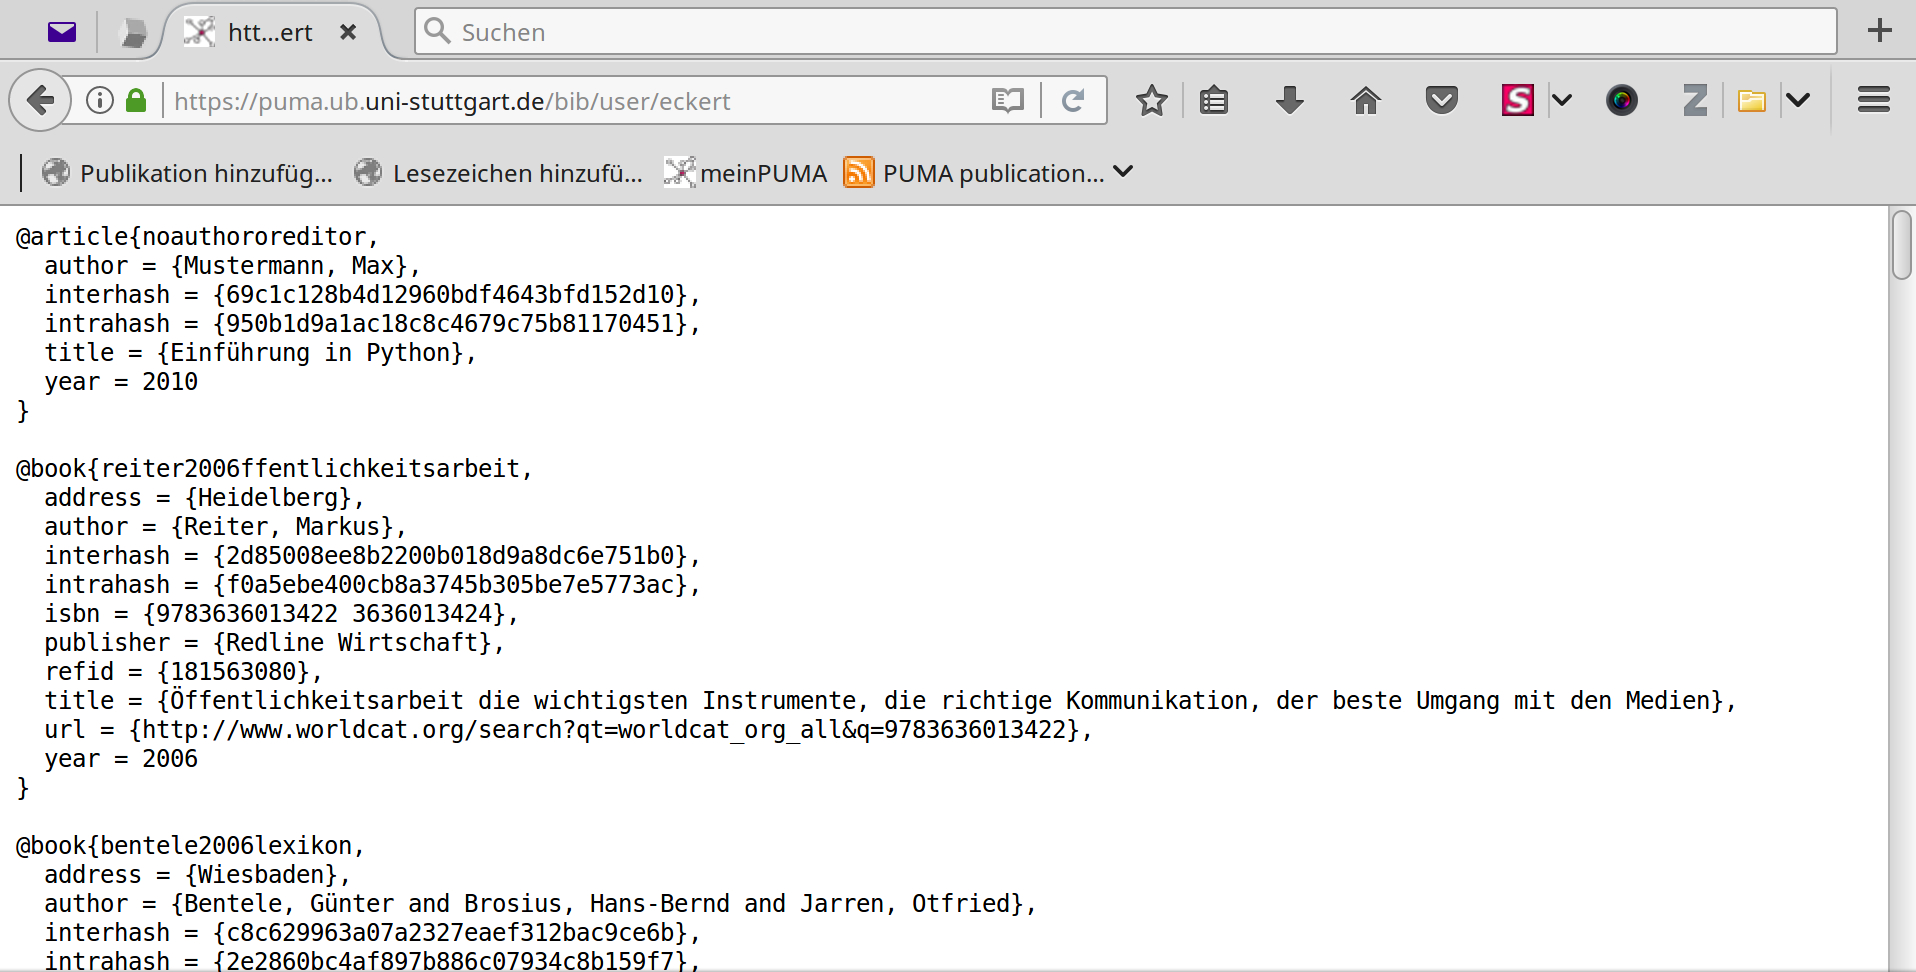
\includegraphics[width=11cm]{Bilder/Kapitel6/Bibtex_Liste}}
 %\caption{BibTex-Liste}
 %\label{figure038}
%\end{figure}
%
%\end{enumerate}
%\subsection{JabRef-Layouts}
%Einen kompletten Überblick zu allen verfügbaren Jabref-Layouts\index{JabRef!Layouts} erhalten Sie auf der Export-Seite von PUMA.
%\begin{enumerate}
	%\item  \textbf{/layout/simplehtml/}\newline
	%Sie erhalten eine HTML-Übersicht - über alle Publikationen im 		Inhaltsbereich - ohne Kopf- oder Fußzeile nützlich für die 			Einbindung von Publikationslisten in andere HTML-Seiten.
	%\item \textbf{/layout/html/}\newline
    %Eine einfache Übersicht aller Publikationen aus dem Inhaltsbereich, in der jeder Eintrag als Zeile in einer Tabelle dargestellt ist.
	%\item \textbf{/layout/tablerefs/} \newline
    %HTML-Ausgabe mit jedem Eintrag als Zeile in einer Tabelle und einer zusätzlichen JavaScript-Suchfunktion.
%\item \textbf{/layout/tablerefsabsbib/} \newline
    %Ähnelt \textit{/layout/tablerefs/}. Enthält auch die BibTeX-Quelle und die Kurzbeschreibung der Publikation.
%\item \textbf{/layout/docbook/} \newline
    %Dies ist eine XML-Ausgabe gemäß dem DocBook-Schema.
%\item \textbf{/layout/endnote/} \newline
    %Sie erhalten eine Ausgabe in RIS, welche von dem Literaturverwaltungsprogramm EndNote verwendet wird.
%\item \textbf{/layout/dblp/} \newline
    %DBLP exportiert alle Publikationen aus dem Inhaltsbereich in eine DBLP-konforme XML-Struktur. 
%\item \textbf{/layout/text/}\newline
    %Alle Publikationen aus dem Inhaltsbereich werden in einer BibTeX-Ausgabe dargestellt.
%\end{enumerate}

\todo[inline]{Sortieren: Datum! Bibtexfelder auswählen Persönlicher Bereich vs. Lucine Index}
\todo[inline]{Dubletten erklären}
